%%%%%%%%%%%%%%%%%%%%%%%%%%%%%%%%%%%%%%%%%%%%%%%%%%%%%%%%%%%%%%%%%%%%%%%%%%%%%%%%
%   Chapter 4
%%%%%%%%%%%%%%%%%%%%%%%%%%%%%%%%%%%%%%%%%%%%%%%%%%%%%%%%%%%%%%%%%%%%%%%%%%%%%%%%
\chapter{Error Propagation in Convoys} \label{chap:errprop}

\section{Introduction} \label{sec:errintro}

% RPV diagram
\begin{figure}[ht] \centering \label{fig:rpvs}
\begin{tikzpicture}[
        scale=3,
        axis/.style={thick, ->, >=stealth'},
        vector/.style={ultra thick, ->, >=stealth'},
        every node/.style={circle, color=black}
    ]
    \draw[axis] (-0.1,0) -- (1.1,0) node(xline)[right] {$E$};
    \draw[axis] (0,-0.1) -- (0,1.1) node(yline)[above] {$N$};
    % points
    \coordinate (a) at (0.25,0.25);
    \coordinate (b) at (0.5,0.75);
    \coordinate (c) at (0.95,0.3);
    \foreach \x in {a,b,c} {
        \node[draw,circle,inner sep=2pt,fill=red] at (\x) {};
    }
    \node [below left] at (a) {$r_1$};
    \node [above] at (b) {$r_2$};
    \node [below right] at (c) {$r_3$};
    % arrows
    \draw[vector] (a) -- (b) node [pos=0.5, sloped, above] {$R_{1,2}$};
    \draw[vector] (b) -- (c) node [pos=0.5, sloped, above] {$R_{2,3}$};
    \draw[vector] (a) -- (c) node [pos=0.5, sloped, below] {$R_{1,3}$};
\end{tikzpicture}
\caption{RPVs used in investigation}
\end{figure}

%%%%% Problem definition
At its simplest, this chapter will examine errors in an RPV resultant from the summantion of multiple intermediate RPVs as compared to an RPV between two points directly. That is, when using DRTK to compute RPVs, how do the errors of $~R_{1,2}+R_{2,3}~$  compare to those of $~R_{1,3}~$? To establish a nomenclature, $R_1$ shall be thought of as a convoy leader, $R_2$ as an intermediate vehicle, and $R_3$ as a following vehicle.


\section{Experimentation}
A one hour data set was taken with three antennas completely static --- meaning a fixed baseline --- 

A half hour data set was recorded with all three antennas at the same baseline as the set described before, but the vehicle on which all three were mounted was driven in chaotic patterns at speeds between $4.5~m/s$ and $13.5~m/s$ in a GPS-benign environment.


\section{Results}

% Fixed baseline Static
\begin{figure}[ht] \centering \label{fig:fixed_static_err_rpv}
    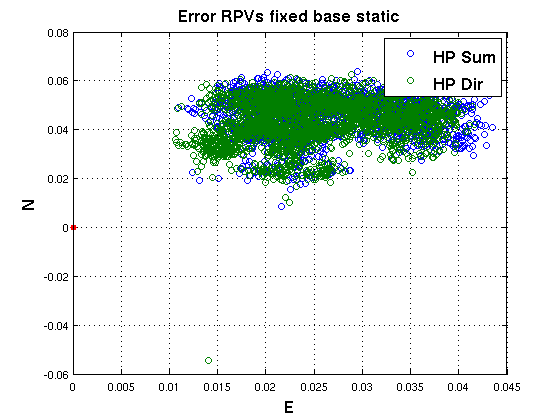
\includegraphics[width=6.5in]{./figs/fixed_static_error_rpv.png}
    \caption{}
\end{figure}

\begin{figure}[ht] \centering \label{fig:fixed_static_err_mag}
    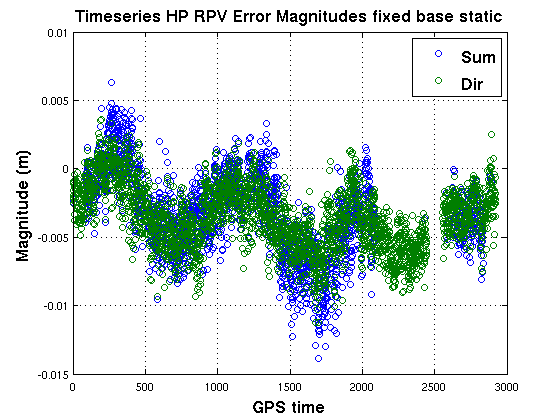
\includegraphics[width=6.5in]{./figs/fixed_static_err_mags.png}
    \caption{}
\end{figure}

% Fixed baseline Dynamic
\begin{figure}[ht] \centering \label{fig:fixed_dynamic_err_rpv}
    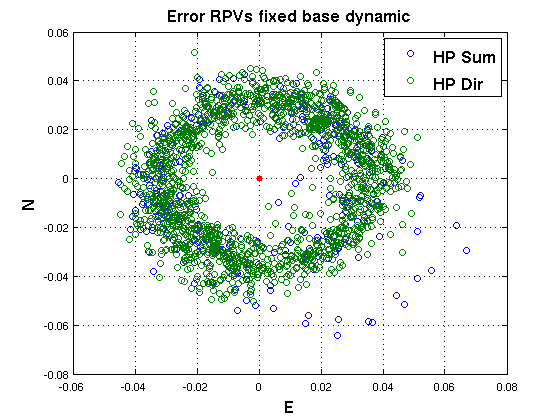
\includegraphics[width=6.5in]{./figs/fixed_dynamic_error_rpv.png}
    \caption{}
\end{figure}

\begin{figure}[ht] \centering \label{fig:fixed_dynamic_err_mag}
    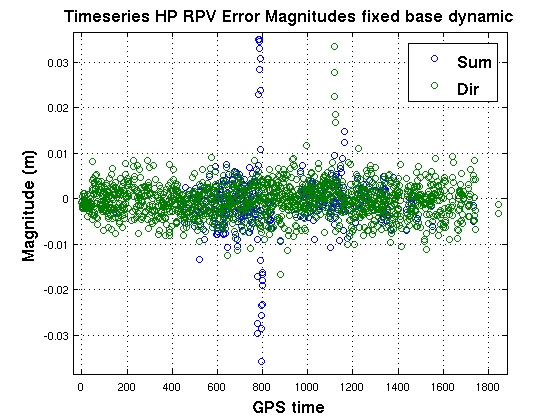
\includegraphics[width=6.5in]{./figs/fixed_dynamic_err_mags.png}
    \caption{}
\end{figure}



% Results table
\begin{table}[htbp] \caption{Statistical Comparison} \centering
\begin{tabular}{r||c|c} \hline
                & Fixed Base, Static  &  Fixed Base, Dynamic \\
    \hline \hline
    Variance, mag of errors & & \\
        Sum (mm): & 0.008 & 0.023 \\
        Dir (mm): & 0.005 & 0.014 \\ \hline
    RMS value of mag errors & & \\
        Sum (mm): & 3.854 & 3.162 \\
        Dir (mm): & 3.684 & 2.810 \\ \hline
\end{tabular} \label{tab:turb_interp} \end{table}

